%As discussed in section \ref{Related work}, t
The most popular techniques to perform itemset mining (e.g.,
Apriori~\cite{Agr94} and FP-growth~\cite{Han00}) adopt the itemset enumeration
approach (see Section \ref{survey_centralized} for further discussion).
% to mine the frequent itemsets.
However, itemset enumeration revealed to be ineffective with datasets with a
high average number of items per transactions \cite{Zaki_Carpenter}.
%Apriori algorithm, in fact, has a very high number of candidates to generate
%and to count, while the trees generated by FP-Growth-based approaches hardly
%fit in main memory.
%In conclusion, these algorithms were not developed for the use cases related
% to high number of features, focusing on high number of transactions.\\
To tackle this problem, the Carpenter algorithm~\cite{Zaki_Carpenter} was
proposed.
Specifically, Carpenter is a frequent itemset extraction algorithm devised to
handle datasets characterized by a relatively small number of
transactions but a huge number of items per transaction.
To efficiently solve the itemset mining problem, Carpenter adopts an effective
depth-first transaction enumeration approach based on the transposed
representation of the input dataset.
To illustrate the centralized version of Carpenter, we will use the running
example dataset $\mathcal{D}$ reported in Figure~\ref{horizontalexampledataset},
and
more specifically, its transposed version (see Figure~\ref{TTexampledataset}).
%Before going deeper into the algorithm explanation, some preliminary
% information will be provided to facilitate the reader comprehension.
%Let us start saying that the algorithm assumes to process a vertical
%transposition of the input dataset.
%Carpenter assumes to process a transposed representation of the input dataset.
Recall that in the transposed
representation each row of the table consists of an item $i$ with its tidlist.
For instance,
the last row of Figure~\ref{TTexampledataset} shows that item \textit{v}
appears in
transactions 1, 2, 3, 4.
%The rows are sorted in a numerical order (oppure The tids in each tidlist are
%sorted in a numerical orders?).
%From the initial transposed table TT, given x as a row or a row set,
%  $x$, $TT|_{x}$, is the projection of the whole vertical datasets on the
%row or the row set $x$, as defined in section \ref{Preliminaries}.\\


\begin{figure}[!t]
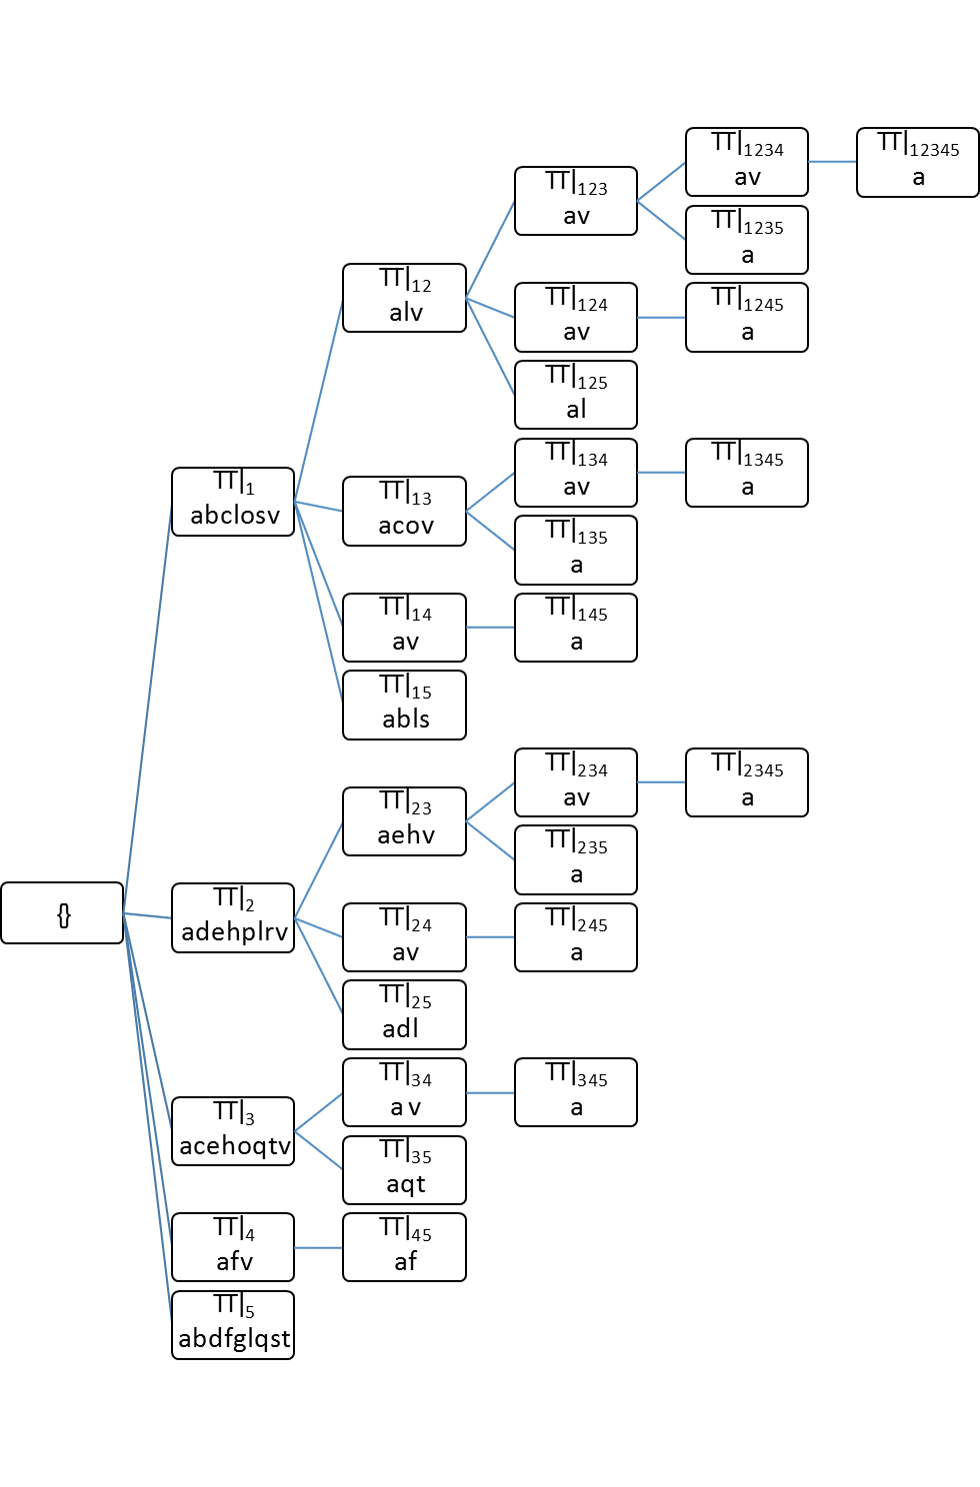
\includegraphics[width=4in]{chapters/pampa/running_example1.png}
\caption{The transaction enumeration tree of the running example dataset in
Figure~\ref{horizontalexampledataset}. For the sake of clarity, no pruning rules
are applied to the tree.}
\label{running_1}
\end{figure}

%Conditional transposed tables and the depth first enumeration of the
%transactions are the core of Carpenter. Specifically,
Basically, Carpenter builds a transaction enumeration tree by exploiting a set of pruning rules
which avoid the expansion of useless branch of the tree. 
In the tree, each node corresponds to a
conditional transposed table $TT|_X$ and its related information (i.e., the
tidlist $X$ with respect to which the conditional transposed table is built and
its associated itemset).
The transaction enumeration tree, when pruning techniques are not applied,
contains all the tid combinations (i.e., all the possible
tidlists $X$).
Figure~\ref{running_1} reports the
transaction enumeration tree obtained by processing the running example dataset.
To avoid the generation of duplicate
tidlists, the transaction enumeration tree is built by exploring the tids in
lexicographical order (e.g., $TT|_{\{1,2\}}$ is generated instead of
$TT|_{\{2,1\}}$).
Each node of the tree is associated with a conditional transposed table on a
tidlist.
For instance, the conditional transposed table
$TT|_{\{2,3\}}$ in Figure~\ref{conditionalexampledataset}, matches the node
$\{2,3\}$ in Figure~\ref{running_1}.


%The enumeration tree is built from initial transposed table: in figure
%\ref{running_1}, a full exploration of the tree based on initial transposed
%table is shown. Each node of the tree, as already said, matches a transposed
%table over a row set. In our example, the transposed table$TT|_{2,3}$ in
%figure 3, matches the node 2,3 in figure \ref{running_1}.
Carpenter performs a depth first search (DFS) of the enumeration tree to mine the set
of frequent closed itemsets.
%Visiting the tree in this way, adopting a pruning branch policy that will
%be detailed in the following, leads to the extraction of the complete
%frequent closed itemset set without duplicates (details and proofs can be
%found in \cite{Zaki_Carpenter}).
%We will describe the Carpenter algorithm by means of the running example.
Referring to the tree in Figure~\ref{running_1}, the depth first search would
lead to the visit of the nodes in the following order:
\{1\}, \{1,2\}, \{1,2,3\}, \{1,2,3,4\}, \{1,2,3,4,5\}, \{1,2,3,5\}, \{...\}.
For each node, Carpenter applies a procedure that decides if the itemset
associated with that node is a frequent closed itemset or not.
%Specifically, for each node, Carpenter decides if the itemset associated with
%the current node is a frequent closed  itemset
%by considering: 1) the tidlist $X$ associated with the node, 2) the conditional
%transposed table
%$TT|_{X}$, 3) the set of frequent closed itemsets found up to the current step
%of the tree search, and 4) the enforced minimum support threshold ($minsup$).
%The first information is useful to enforce the DFS exploration and to check the 
%actual support of the itemset; the conditional transposed table is used to obtain
% the itemset associated to the node, while the remaing tids are useful to determine
% how and if the node should be expanded. The frequent closed itemsets found (3)
% are used to avoid to process the same itemset twice; due to the enumeration tree 
%architecture, the real support of the itemset is the one obtained the first time the 
%itemset is processed in a DFS exploration manner. Finally, the enforced minsup 
%support threshold is used to decide if the itemset is a frequent closed itemset.
Specifically, for each node, Carpenter decides if the itemset associated with
the current node is a frequent closed  itemset
by considering: \begin{enumerate}
\item The tidlist $X$ associated with the node, useful to enforce the depth-first exploration and to check the actual support of the itemset
\item The conditional transposed table $TT|_{X}$, used to obtain the itemset associated to the node and, through the remaing tids, determine how and if the node should be expanded
\item The set of itemsets found up to the current step of the tree search, used to avoid to process the same itemset twice (due to the enumeration tree architecture, the real support of the itemset is the one obtained the first time the itemset is processed in a depth-first exploration manner)
\item The enforced minimum support threshold ($minsup$), used to decide if the itemset is a frequent closed itemset
\end{enumerate}
Based on the theorems reported in~\cite{Zaki_Carpenter}, if the itemset $I$
associated with the current node is a frequent closed itemset then $I$
is included in the frequent closed itemset set. Moreover, by exploiting the
analysis performed on the current node, part of the remaining search space
(i.e.,
part of the enumeration tree) can be pruned, to avoid the analysis of nodes that
will never generate new closed itemsets.
To this purpose, three pruning rules are applied on the enumeration tree, based
on the evaluation performed on the current node and the associated
transposed table $TT|_{X}$:
\begin{itemize}
\item \textbf{Pruning rule 1.} If the size of $X$, plus the number of distinct
tids in the rows of $TT|_{X}$ does not reach the minimum support threshold,
the subtree rooted in the current node is pruned.
\item \textbf{Pruning rule 2.} If there is any tid $tid_i$ that is present in
all the tidlists of the rows of $TT|_{X}$, $tid_i$ is deleted from $TT|_{X}$.
The number of discarded tids is updated to compute the correct support of the
itemset associated with the pruned version of $TT|_{X}$.
\item \textbf{Pruning rule 3.} If the itemset associated with the current node
has been already encountered during the depth first search,
the subtree rooted in the current node is pruned because it can never generate
new closed itemsets.
\end{itemize}

%Rule 3 is the most effective pruning rule, especially considering the
%distributed implementation detailed in \ref{Distributed implementation
%outline}. It allows to prune the branches related to already found itemsets,
%that represents a waste of computation time and memory.
%After the pruning phase, the support of the itemset is compared with the
%minsup. The support is identified by the number of row ids composing $X$,
%plus the number of rows discarded by the second pruning rule. If the support
%is greater or equal than the minsup, as shown in figure 5, the itemset
%is added to the set of frequent closed ones.

The tree search continues in a depth first fashion moving on the next node of
the enumeration tree. More specifically,
let $tid_l$ be the lowest tid in the tidlists of the current $TT|_{X}$, the next
node to explore is the one associated with
$X^\prime=X\cup \{tid_l\}$.


Among the three rules mentioned above, pruning rule 3 assumes a global knowledge
of the enumeration tree explored in a depth first manner.
This, as detailed in section~\ref{Distributed implementation outline}, is very
challenging in a distributed environment that adopts a shared-nothing
architecture, like the one we address in this work.



% %versione 2
% %\\
% %Carpenter algorithm is based on the depth first exploration of a row
% enumeration tree. A running example of the enumeration tree built on the dataset
% in table 1 is represented in figure \ref{running_1}. A transposed table
% $TT|_{x}$ is the projection of the whole vertical datasets on the row set x, as
% defined in \ref{Preliminaries}. Each transposed table is associated with an
% itemset composed of the items in the table. For each item, the associated
% tidlist is composed of the tids greater than any tid in the row set x. Each
% table represents a node in the row enumeration tree. For instance, $TT|_{2,3}$
% in tab 3 corresponds to the node 2 3 in the enumeration tree.
% %\\The tree exploration corresponds to a recursive processing of the transposed
% tables, generating adding a tid to the row set in depth first manner. Exploring
% the tree in this way, applying a set of pruning rules detailed in a few lines,
% leads to the extraction of all the closed itemsets (details and proofs can be
% found in \cite{Zaki_Carpenter}). The first iteration processes the whole
% vertical dataset. Each iteration, given a transposed table $TT|_{x}$ as input,
% can be resumed in:
% %\begin{enumerate}
% %\item apply pruning rules
% %\item if the support is over the minsup, add the related itemset to the set of
% frequent closed itemsets
% %\item expand the table adding a tid in the row set, following a depth first
% manner
% %\item start a new recursion with the new table
% %\end{enumerate}
% %The pruning rules allow to prune some branches without exploring all the
% possible tid combinations. The most effective is the rule used to prune some
% branches of the tree if the related itemsets have already been found in the tree
% exploration. The rules are:
% %\begin{itemize}
% %\item \textbf{Pruning rule 1:} If the row of the projection, plus the potential
% rows in the tid lists do not reach the minimum support threshold, the table is
% discarded and the branch is pruned.
% %\item \textbf{Pruning rule 2:} If there is any row id which is present in all
% the tid lists, it is deleted from the table. The number of discarded rows is
% updated.
% %\item \textbf{Pruning rule 3:} If the itemset characterizing the table has been
% already seen in the tree, the branch is pruned.
% %\end{itemize}
% %The process continues recursively until there is no table to expand and all the
% closed itemsets have been found. A most detailed explanation and theoretical
% proofs are in \cite{Zaki_Carpenter}.

\begin{figure}[!t]
%\centering
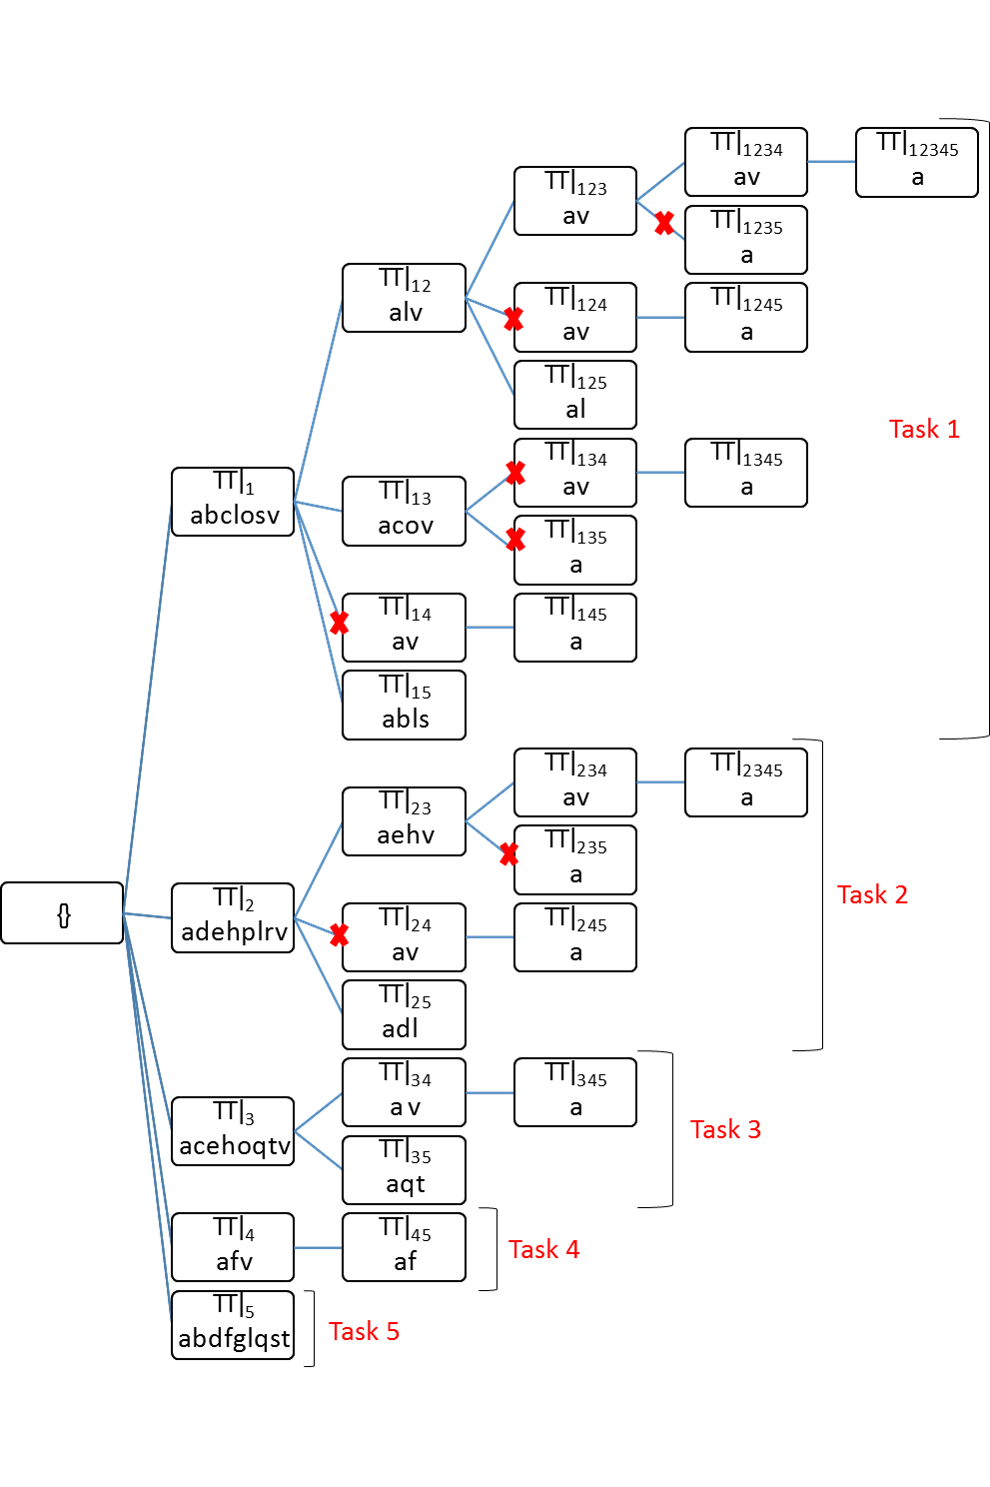
\includegraphics[width=4in]{chapters/pampa/running_example2_d.png}
% where an .eps filename suffix will be assumed under latex,
% and a .pdf suffix will be assumed for pdflatex; or what has been declared
% via \DeclareGraphicsExtensions.
\caption{Running toy example: each node expands a branch of the tree
independently. For the sake of clarity, pruning rule 1 and 2 are not applied. The pruning rule 3 is
applied only within the same task: the small crosses on the edges represent pruned
nodes due to local pruning rule 3, e.g.
the one on node \{2 4\} represents the pruning of node \{2 4\}.}
\label{running_2}
\end{figure}

